\documentclass[12pt, oneside]{article}
\usepackage{amsmath}
\usepackage{amssymb}
\usepackage{amsfonts}
\usepackage{graphicx}
\usepackage{listings}
\usepackage[margin=1in]{geometry}
\usepackage[normalem]{ulem}
\usepackage{latexsym}
\usepackage{xcolor}
\usepackage{color}
\usepackage{float}
\usepackage{hyperref}
\usepackage{tikz}
\usepackage{pgfplots}
\usepackage{pgfplotstable}
\usepackage{booktabs}
\usepackage{multirow}
\usepackage{siunitx}
\usepackage{enumitem}
\usepackage{subcaption}
\usepackage{caption}
\usepackage{cleveref}
\usepackage{mathtools}
\usepackage{bm}
\usepackage{algpseudocode}
\usepackage{algorithmicx}
\usepackage{tcolorbox}

\usepackage[letterpaper, scale=0.89, centering]{geometry}
\usepackage{fancyhdr}
\setlength{\parindent}{0em}
\setlength{\parskip}{1em}

\usepackage{tikz}
\usetikzlibrary{automata,positioning,arrows}

\pagestyle{fancy}
\fancyhf{}
\renewcommand{\headrulewidth}{0pt}
\rfoot{\href{https://creativecommons.org/licenses/by-nc-sa/2.0/}{CC BY-NC-SA 2.0} Version \today~(\thepage)}

\usepackage{amssymb,amsmath,pifont,amsfonts,comment,enumerate,enumitem}
\usepackage{currfile,xstring,hyperref,tabularx,graphicx,wasysym}
\usepackage[labelformat=empty]{caption}
\usepackage{xcolor}
\usepackage{multicol,multirow,array,listings,tabularx,lastpage,textcomp,booktabs}

\lstnewenvironment{algorithm}[1][] {   
    \lstset{ mathescape=true,
        frame=tB,
        numbers=left, 
        numberstyle=\tiny,
        basicstyle=\rmfamily\scriptsize, 
        keywordstyle=\color{black}\bfseries,
        keywords={,procedure, div, for, to, input, output, return, datatype, function, in, if, else, foreach, while, begin, end, }
        numbers=left,
        xleftmargin=.04\textwidth,
        #1
    }
}
{}

\newcommand\abs[1]{\lvert~#1~\rvert}
\newcommand{\st}{\mid}

\newcommand{\cmark}{\ding{51}}
\newcommand{\xmark}{\ding{55}}
\newcommand{\answer[1]}{\\[#1]\\}
\newcommand{\tab}{~~~~}
\begin{document}

Welcome to CSE 105: Introduction to Theory of Computation in Fall 2024!

\section*{CSE 105's Big Questions}
\begin{itemize}
   \item What problems are computers capable of solving?
   \item What resources are needed to solve a problem?
   \item Are some problems harder than others?
\end{itemize}

In this context, a {\bf problem} is defined as: ``Making a decision or computing a value based on some input"

Consider the following problems: 
\begin{itemize}
   \item Find a file on your computer
   \item Determine if your code will compile - easiest
   \item Find a run-time error in your code
   \item Certify that your system is un-hackable - hardest
\end{itemize}

Which of these is hardest?

In Computer Science, we operationalize ``hardest'' as ``requires most resources'', where
resources might be memory, time, parallelism, randomness, power, etc.

To be able to compare ``hardness'' of problems, we use a consistent description of problems

{\bf Input}: String

{\bf Output}: Yes/ No, where Yes means that the input string matches the pattern or property described by the problem.

\newpage

\subsection*{Weeks 0 and 1 at a glance}

\subsubsection*{Textbook reading: Chapter 0, Sections 1.3, 1.1}

\vspace{-15pt}

Before Monday, review class syllabus on Canvas (https://canvas.ucsd.edu/) and 
read Example 1.51 and Definition 1.52 (definition of regular expressions) on page 64.
{\it Notice}: we are jumping to Section 1.3 and then will come back 
to Section 1.1 on Wednesday.

Before Wednesday, read Figure 1.4 and Definition 1.5 (definition of finite automata) on pages 34-35.

Before Friday, read the definition of the union, concatenation, and star operations for languages is given 
as Definition 1.23 on page 44 and a useful example is Example 1.24.

For Week 2 Monday: Pages 41-43 (Figures 1.18, 1.19, 1.20) (examples of automata and languages).


{\it Textbook references: Within a chapter, each item is numbered consecutively. Figure 1.22
is the twenty-second numbered item in chapter one; it comes right after Example 1.21 and right before Definition 1.23.}


\subsubsection*{We will be learning and practicing to:}
\begin{itemize}
\item Clearly and unambiguously communicate computational ideas using appropriate formalism. Translate across levels of abstraction.
\begin{itemize}
   \item Translate a decision problem to a set of strings coding the problem.
   \begin{itemize}
   \item {\bf Distinguish between alphabet, language, sets, and strings}
   \end{itemize}
   \item Use regular expressions and relate them to languages and automata.
   \begin{itemize}
      \item {\bf Write and debug regular expressions using correct syntax}
      \item {\bf Determine if a given string is in the language described by a regular expression}
   \end{itemize}
   \item Use precise notation to formally define the state diagram of finite automata.
   \item Use clear English to describe computations of finite automata TM informally.
   \begin{itemize}
      \item {\bf State the formal definition of (deterministic) finite automata}   
      \item {\bf Trace the computation of a finite automaton on a given string using its state diagram}
      \item {\bf Translate between a state diagram and a formal definition}
      \item {\bf Determine if a given string is in the language recognized by a finite automaton}
   \end{itemize}
\end{itemize}




\end{itemize}

\subsubsection*{TODO:}
\begin{list}{\itemsep-10pt}
   \item \#FinAid Assignment on Canvas (complete as soon as possible) and read syllabus on Canvas
   \item Schedule your Test 1 Attempt 1, Test 2 Attempt 1, Test 1 Attempt 2, and Test 2 Attempt 2 times 
   at PrairieTest (http://us.prairietest.com)
   \item Review Quiz on PrairieLearn (http://us.prairielearn.com), complete by Sunday 10/6/2024
   \item Create a homework group, possibly by using the Piazza (https://piazza.com/) find-a-teammate tool
   \item Homework 1 submitted via Gradescope (https://www.gradescope.com/), due Tuesday 10/8/2024
\end{list}

\newpage

\section*{Week 0 Friday: Terminology and Notation}



The CSE 105 vocabulary and notation build on discrete
math and introduction to proofs classes.  Some of the conventions may 
be a bit different from what you saw before so we'll draw your attention to them.

For consistency, we will use the notation from this class' textbook\footnote{Page references are to 
the 3rd edition of Sipser's Introduction to the Theory of Computation,
available through various sources for approximately \$30. You may be able to 
opt in to purchase a digital copy through Canvas. Copies of the book are also available 
for those who can't access the book
to borrow from the course instructor, while supplies last (minnes@ucsd.edu)}.

These definitions are on pages 3, 4, 6, 13, 14, 53.

\begin{center}
    \begin{tabular}{|p{2.6in}cp{3.5in}|}
    \hline 
    {\bf Term} & {\bf Typical symbol} & {\bf Meaning} \\
     & or {\bf Notation} & \\
    \hline
    && \\
    Alphabet & $\Sigma$, $\Gamma$ & A non-empty finite set	 \\
    Symbol over $\Sigma$  & $\sigma$, $b$, $x$ & An element of the alphabet $\Sigma$\\ 
    String over $\Sigma$  &	$u$, $v$, $w$ & A finite list of symbols from $\Sigma$\\
    (The) empty string &$\varepsilon$ & The (only) string of length $0$\\
    The set of all strings over $\Sigma$ & $\Sigma^*$ & The collection of all possible strings formed from symbols from $\Sigma$ \\ 
    (Some) language over $\Sigma$& $L$ & (Some) set of strings over $\Sigma$ \\ 
    (The) empty language &$\emptyset$ & The empty set, i.e. the set that has no strings (and no other elements either)\\
    && \\
    \hline
    && \\
    The power set of a set $X$ &$\mathcal{P}(X)$ & The set of all subsets of $X$ \\
    (The set of) natural numbers &$\mathcal{N}$ & The set of positive integers \\ 
    (Some) finite set & & The empty set or a set whose distinct elements can be counted by a natural number\\
    (Some) infinite set & & A set that is not finite.\\ 
    &&\\
    \hline
    && \\
    Reverse of a string $w$ & $w^\mathcal{R}$  & write $w$  in  the opposite order, if $w = w_1 \cdots  w_n$ then $w^\mathcal{R} = w_n \cdots  w_1$. Note: $\varepsilon^\mathcal{R} = \varepsilon$\\
    Concatenating strings $x$ and $y$ & $xy$ &  take $x = x_1 \cdots x_m$, $y=y_1 \cdots y_n$ and form $xy = x_1 \cdots x_m y_1 \cdots y_n$\\
    String $z$ is a substring of string $w$ & & there are strings $u,v$ such that $w = uzv$\\
    String $x$ is a prefix of string $y$ & & there is a string $z$ such that $y = xz$ \\
    String $x$ is a proper prefix of string $y$ & & $x$ is a prefix of $y$ and $x \neq y$\\
    && \\
    \hline
    &&\\
    Shortlex order, also known as string order over alphabet $\Sigma$ & & Order strings over  $\Sigma$ first 
    by length and then according to the dictionary order, assuming symbols in $\Sigma$  have an ordering\\ \hline
    \end{tabular}
\end{center}

\vfill
    
\newpage
Write out in words the meaning of the symbols below: 

\[
    \{ a, b, c\}
\]

\phantom{The set whose elements are $a$, $b$, and $c$}

\[
    | \{a, b, a \} | = 2
\]

\phantom{The number of elements in the set $\{a,b,a\}$ is $2$.}

\[
    | aba | = 3
\]

\phantom{The length of the string $aba$ is $3$.}

\begin{comment}

\[
    (a, 3, 2, b, b)
\]

\phantom{The $5$-tuple whose first components is $a$, second component 
is $3$, third component is $2$, fourth component is $b$, and fifth component is $b$.}
\end{comment}

{\it Circle the correct choice}:

A {\bf string} over an alphabet $\Sigma$ is \underline{~~an element of $\Sigma^*$ ~~ OR ~~ a subset of $\Sigma^*$}.
    
A {\bf language} over an alphabet $\Sigma$ is \underline{~~an element of $\Sigma^*$ ~~ OR ~~ a subset of $\Sigma^*$}.


With $\Sigma_1 = \{0,1\}$ and 
$\Sigma_2 = \{a,b,c,d,e,f,g,h,i,j,k,l,m,n,o,p,q,r,s,t,u,v,w,x,y,z\}$
and $\Gamma = \{0,1,x,y,z\}$

{\bf True} or {\bf False}: $\varepsilon \in \Sigma_1$

{\bf True} or {\bf False}: $\varepsilon$ is  a string over $\Sigma_1$

{\bf True} or {\bf False}: $\varepsilon$ is a language over $\Sigma_1$

{\bf True} or {\bf False}: $\varepsilon$ is a prefix of some string over  $\Sigma_1$

{\bf True} or {\bf False}: There is a string over $\Sigma_1$ that is a proper prefix of $\varepsilon$
    

The first five strings over $\Sigma_1$ in string order, using the ordering $0 <  1$: \\
$\epsilon, 0, 1, 00, 01$
    
The first five strings over $\Sigma_2$ in string order, using the usual alphabetical ordering for single letters:\\
$\epsilon, a, b, c, d$
     
\newpage

\section*{Week 1 Monday: Regular expressions}

Our motivation in studying sets of strings is that they can be used to encode problems.
To calibrate how difficult a problem is to solve, we describe how complicated the set of strings that encodes it is. 
How do we define sets of strings?\\

Set notation: $\{\}$\\
Roster notation: ex. $\{a, b, c\}$ -- works for finite sets\\ 
Set builder notation: ex. $\{ x \mid P(x)\}$ -- works for infinite sets or $\{ f(x) \mid x\}$\\
Named sets: ex. $\mathbb{N}$, $\mathbb{Z}$, $\emptyset$\\
Recursive/Inductive definitions: Basis steps, and recursive step\\


How would you describe the language that has no elements at all?\\

Given an alphabet, the language is the set of strings over that alphabet\\
The language with no elements can be described as $\{\}$ or $\emptyset$ or $\{ x \in \Sigma \mid x \neq x \}$\\

How would you describe the language that has all strings over $\{0,1\}$ as its elements?\\

Can easily be done recursively: \\
Base step: $\varepsilon \in L$\\
Recursive step: if $w \in \Sigma^*$, then $0w, 1w \in \Sigma^*$\\\\

Kleene star set operation: for any set $A$, $A^* = \{ w_1 \cdots w_k \mid k \geq 0 \textrm{ and each } w_i \in A\}$\\

\newpage

**This definition was in the pre-class reading**
{\bf Definition 1.52}: A {\bf regular expression} over alphabet $\Sigma$ is a syntactic expression that can describe 
a language over $\Sigma$. The collection of all regular expressions over $\Sigma$ is defined recursively:
\begin{itemize}
\item[] {\it Basis steps of recursive definition}
\begin{quote}    
    $a$ is a regular expression, for $a \in \Sigma$

    $\varepsilon$ is a regular expression

    $\emptyset$ is a regular expression
\end{quote}

\item[] {\it Recursive steps of recursive definition}
\begin{quote}
    $(R_1 \cup R_2)$ is a regular expression when $R_1$, $R_2$ are regular expressions 

    $(R_1 \circ R_2)$ is a regular expression when $R_1$, $R_2$ are regular expressions

    $(R_1^*)$ is a regular expression when $R_1$ is a regular expression 
\end{quote}
\end{itemize}
 

The {\it semantics} (or meaning) of the syntactic regular expression is the {\bf language
described by the regular expression}. The function that assigns a language to a regular expression
over $\Sigma$ is defined recursively, using familiar set operations:


\begin{itemize}
    \item[] {\it Basis steps of recursive definition}
    \begin{quote}    
        The language described by $a$, for $a \in \Sigma$, is $\{a\}$ and we write 
        $L(a) = \{a\}$
    
        The language described by $\varepsilon$ is $\{\varepsilon\}$ and we write 
        $L(\varepsilon) = \{ \varepsilon\}$
    
        The language described by $\emptyset$ is $\{\}$ and we write
        $L(\emptyset) = \emptyset$.
    \end{quote}
    A language has to have all of its elements be strings\\
    
    \item[] {\it Recursive steps of recursive definition}
    \begin{quote}
        When $R_1$, $R_2$ are regular expressions, the language described by the regular
        expression $(R_1 \cup R_2)$ is the union of the languages described by $R_1$ and $R_2$, 
        and we write 
        $$L(~(R_1 \cup R_2)~) = L(R_1) \cup L(R_2) = \{ w \mid w \in L(R_1) \lor w \in L(R_2)\}$$
    
        When $R_1$, $R_2$ are regular expressions, the language described by the regular
        expression $(R_1 \circ R_2)$ is the concatenation of the languages described by $R_1$ and $R_2$, 
        and we write 
        $$L(~(R_1 \circ R_2)~) = L(R_1) \circ L(R_2) = \{ uv \mid u \in L(R_1) \land v \in L(R_2)\}$$
    
        When $R_1$ is a regular expression, the language described by the regular 
        expression $(R_1^*)$ is the {\bf Kleene star} of the language described by $R_1$ and we write
        $$L(~(R_1^*)~) = (~L(R_1)~)^* = \{ w_1 \cdots w_k \mid k \geq 0 \textrm{ and each } w_i \in L(R_1)\}$$
    \end{quote}
\end{itemize}
  
\newpage
For the following examples assume the alphabet is $\Sigma_1 =  \{0,1\}$:
    
The language described by the regular expression $0$ is $L(0) = \{ 0 \}$\\

The language described by the regular expression $1$ is $L(1)  = \{ 1 \}$

The language described by the regular expression $\varepsilon$ is $L(\varepsilon) = \{ \varepsilon  \}$

The language described by the regular expression $\emptyset$ is $L(\emptyset) = \emptyset$

The language described by the regular expression $(\Sigma_1 \Sigma_1 \Sigma_1)^*$ 
is $L(~(\Sigma_1 \Sigma_1 \Sigma_1)^*~) = $\\
$\Sigma_1$ is the regular expression $(0 \cup 1)$\\
3-length strings over $\Sigma_1$ is the regular expression $(0 \cup 1)(0 \cup 1)(0 \cup 1)$\\
multiple of 3-length strings over $\Sigma_1$ is the regular expression $(0 \cup 1)(0 \cup 1)(0 \cup 1)^*$\\

\vfill

The language described by the regular expression $1^* \circ 1$ is $L(1^* \circ 1) = $

\vfill
     
\newpage

\subsection*{Week 1 Wednesday: Regular expressions conventions}




{\bf Review}: Determine whether each statement below about regular expressions
over the alphabet $\{a,b,c\}$ is true or false:

\begin{comment}
True or False: \qquad 
   $a  \in L(~(a \cup b )~\cup c)$
\end{comment}

True or False: \qquad 
   $ab  \in L(~ (a \cup b)^*  ~)$
   
True or False: \qquad    
   $ba \in L( ~ a^* b^* ~)$
   
True or False: \qquad 
   $\varepsilon  \in L(a \cup b \cup c)$
   
True or False: \qquad 
   $\varepsilon  \in L(~ (a \cup b)^*  ~)$

True or False: \qquad 
   $\varepsilon \in L( ~ aa^* \cup bb^* ~)$

\vfill

{\it Shorthand and conventions} (Sipser pages 63-65)

\vspace{-20pt}

\begin{center}
    \begin{tabular}{|ll|}
    \hline
    & \\
    \multicolumn{2}{|l|}{Assuming $\Sigma$ is the alphabet, we use the following conventions}\\
    & \\
    $\Sigma$   & regular  expression describing language consisting of  all strings  of length  $1$ over $\Sigma$\\
    $*$ then $\circ$ then $\cup$   & precedence order, unless parentheses are used to change it\\
    $R_1R_2$ & shorthand  for  $R_1  \circ R_2$ (concatenation symbol is implicit) \\
    $R^+$ & shorthand for $R^* \circ R$ \\
    $R^k$ & shorthand for $R$ concatenated with itself $k$ times, where $k$ is a (specific) natural number\\
    & \\
    \hline
    \end{tabular}
\end{center}

\vfill 

{\bf Caution: many programming languages that support regular expressions build in functionality
that is more powerful than the ``pure'' definition of regular expressions given here. }

Regular expressions are everywhere (once you start looking for them).

Software tools and languages often have built-in support for regular expressions to describe
{\bf patterns} that we want to match (e.g. Excel/ Sheets, grep, Perl, python, Java, Ruby).

Under the hood, the first phase of {\bf compilers} is to transform the strings we write 
in code to tokens (keywords, operators, identifiers, literals). Compilers use regular expressions
to describe the sets of strings that can be used for each token type.

Next time: we'll start to see how to build machines that decide whether strings match the pattern
described by a regular expression.

\newpage

Practice with the regular expressions over $\{a,b\}$ below.

For example: Which regular expression(s) below describe a language that includes the string $a$ as an element?

$a^* b^*$ 

\vfill

$a(ba)^* b$

\vfill

$a^* \cup b^*$

\vfill

$(aaa)^*$

\vfill

$(\varepsilon \cup a) b$

\vfill 

\newpage
\subsection*{Week 1 Friday: Finite automata}




**This definition was in the pre-class reading**
A finite automaton (FA) is specified by  $M = (Q, \Sigma, \delta, q_0, F)$.
This $5$-tuple is called the {\bf formal definition} of the FA. The FA can also 
be represented by its state diagram: with nodes for the state, labelled edges specifying the 
transition function, and decorations on nodes denoting the start and accept states.

\begin{quote}
Finite set of states $Q$ can be labelled by any collection of distinct names. Often
we use default state labels $q0, q1, \ldots$ 
\end{quote}

\begin{quote}  
The alphabet $\Sigma$ determines the possible inputs to the automaton. 
Each input to the automaton is a string over  $\Sigma$, and the automaton ``processes'' the input
one symbol (or character) at a time.
\end{quote}

\begin{quote}
The transition function $\delta$ gives the next state of the automaton based on the current state of 
the machine and on the next input symbol.
\end{quote}

\begin{quote}
The start state $q_0$ is an element of $Q$.  Each computation of the machine starts at the  start  state.
\end{quote}

\begin{quote}
The accept (final) states $F$ form a subset of the states of the automaton, $F \subseteq  Q$. 
These states are used to flag if the machine accepts or rejects an input string.
\end{quote}


\begin{quote}
The computation of a machine on an input string is a sequence of states
in the machine,  starting with the start state, determined by transitions 
of the machine as it reads successive input symbols.
\end{quote}

\begin{quote}
The finite automaton $M$ accepts the given input string exactly when the computation of $M$ on the input string
ends in an accept state. $M$ rejects the given input string exactly when the computation of 
$M$ on the input string ends in a nonaccept state, that is, a state that is not in $F$.
\end{quote}

\begin{quote} 
The language of $M$, $L(M)$, is defined as the set of  all strings that are each accepted 
by the machine $M$. Each string that is rejected by $M$ is not in $L(M)$.
The language of $M$ is also called the language recognized by $M$.
\end{quote}   
   
What is {\bf finite} about all finite automata? (Select all that apply)
\begin{itemize}
   \item[$\square$] The size of the machine (number of states, number of arrows)
   \item[$\square$] The length of each computation of the machine
   \item[$\square$] The number of strings that are accepted by the machine
\end{itemize}
\newpage
  
\begin{figure}[h]
   \centering
   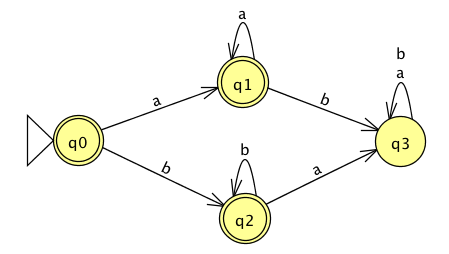
\includegraphics[width=3in]{Lect2DFA1.png} 
\end{figure}
   
The formal definition of this FA is
   
\vfill
\vfill
   

Classify each string $a, aa, ab, ba, bb, \varepsilon$ as accepted by the FA or rejected by the FA.  

{\it Why are these the only two options?}

\vspace{200pt}


The language recognized by this automaton is
  

\vfill

\newpage

\begin{figure}[h]
  \centering
  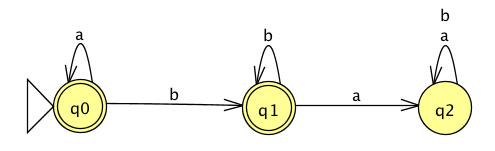
\includegraphics[width=3in]{Lect2DFA2.png} 
\end{figure}
   

The language recognized by this automaton is
  


\vfill

\hrule

\begin{figure}[h]
    \centering
    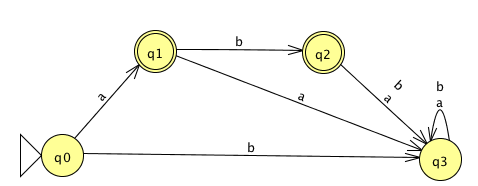
\includegraphics[width=3in]{Lect2DFA3.png} 
\end{figure}

The language recognized by this automaton is
  

\vfill 


\end{document}
